\chapter{Theoretische Betrachtung}
\section{\acl{CMS}}
Ein \ac{CMS} verwaltet die Erstellung und Modifiation von digitalen Inhalten mit
mehreren Nutzern in einem kollabarativen Umfeld.
\subsection{\acl{CMA}}
\ac{CMA} beschreibt den Frontend Part von einem \ac{CMS}. Typischerweise besteht
es aus einer Benutzoberfläche zum Verfassen und Verwalten von digiatalen
Inhalten mithilfe eines \ac{WYSIWYG} Editors. Mithilfe eines solchen Editors ist
es möglich, Inhalte für Webseiten zu erstellen, ohne Sprachen wie \ac{HTML} zu verwenden.
\subsection{\acl{CDA}}
Eine \ac{CDA} beschreibt das Backend, das heißt den Server, auf dem digatle
Inhalte gespeichert, gecached und abgerufen werden können.
\subsection{Bestehende Lösungen}
Es existieren diverse \ac{CMS} Implementationen. Im folgenden werden
zwei betrachtet.
\subsubsection{Wordpress}
Worpress ist eine freie und Open-source \ac{CMS} Implementation von der Worpress
Foundation.\footnote{https://wordpress.org/} Laut ``Built With'' verwenden zum
Zeitpunkt dieser Arbeit 48\% der Webseiten mit einem \ac{CMS}
Wordpress.\footnote{https://trends.builtwith.com/cms abgerufen am 24.05.2019} Dies
macht es zur am weitesten verbreiteten \ac{CMS} Lösung.\\
Als Technologien werden
PHP und Javascript verwendet und durch eine große Anzahl an Plug-ins kann das
\ac{CMS} beliebig erweitert werden.
\subsubsection{Kentico CMS}
Im Gegensatz zu Wordpress ist Kentico CMS eine properitäre Software.\footnote{https://www.kentico.com/product/kentico12} Entwicklet
von Kentico Software seit dem Jahre 2006 bietet das \ac{CMS} unter anderem Funktionen zur
Verwaltung von digitalen Inhalten, E-commerce und für Online Marketing.\\
Bei Kentico kamen C\# und die ASP.NET Plattform zum Einsatz.

% TODO write about MVC and MVVM
\section{\acs{MVC}}
\section{\acs{MVVM}}

\section{\acl{DOM}}
\subsection{Standards}
\ac{XML} bildet eine Dokumenthierarchie ab, welche einen maschinell lesbaren Aufbau eines
Dokumentes, mithilfe von einer generischen Syntax, definiert. \ac{XML} wird in
verschiedenen Formen in vielen Geräten und Programmen genutzt um Datenstrukturen
abzubilden. Diese Datenstrukturen können in verschiedenen, Domäne-spezifischen
varianten beschrieben werden, wie zum Beispiel

\begin{itemize}
\item Scalable Vector Graphic (SVG)
\item Rich Site Summary (RSS)
\item Extensible Hypertext Markup Language (XHTML)
\end{itemize}

Das \ac{DOM} definiert ein \ac{API} zum manipulieren von \ac{XML} als
Baumstruktur. \cite{harold}

\subsection{Aufbau}
\begin{figure}
  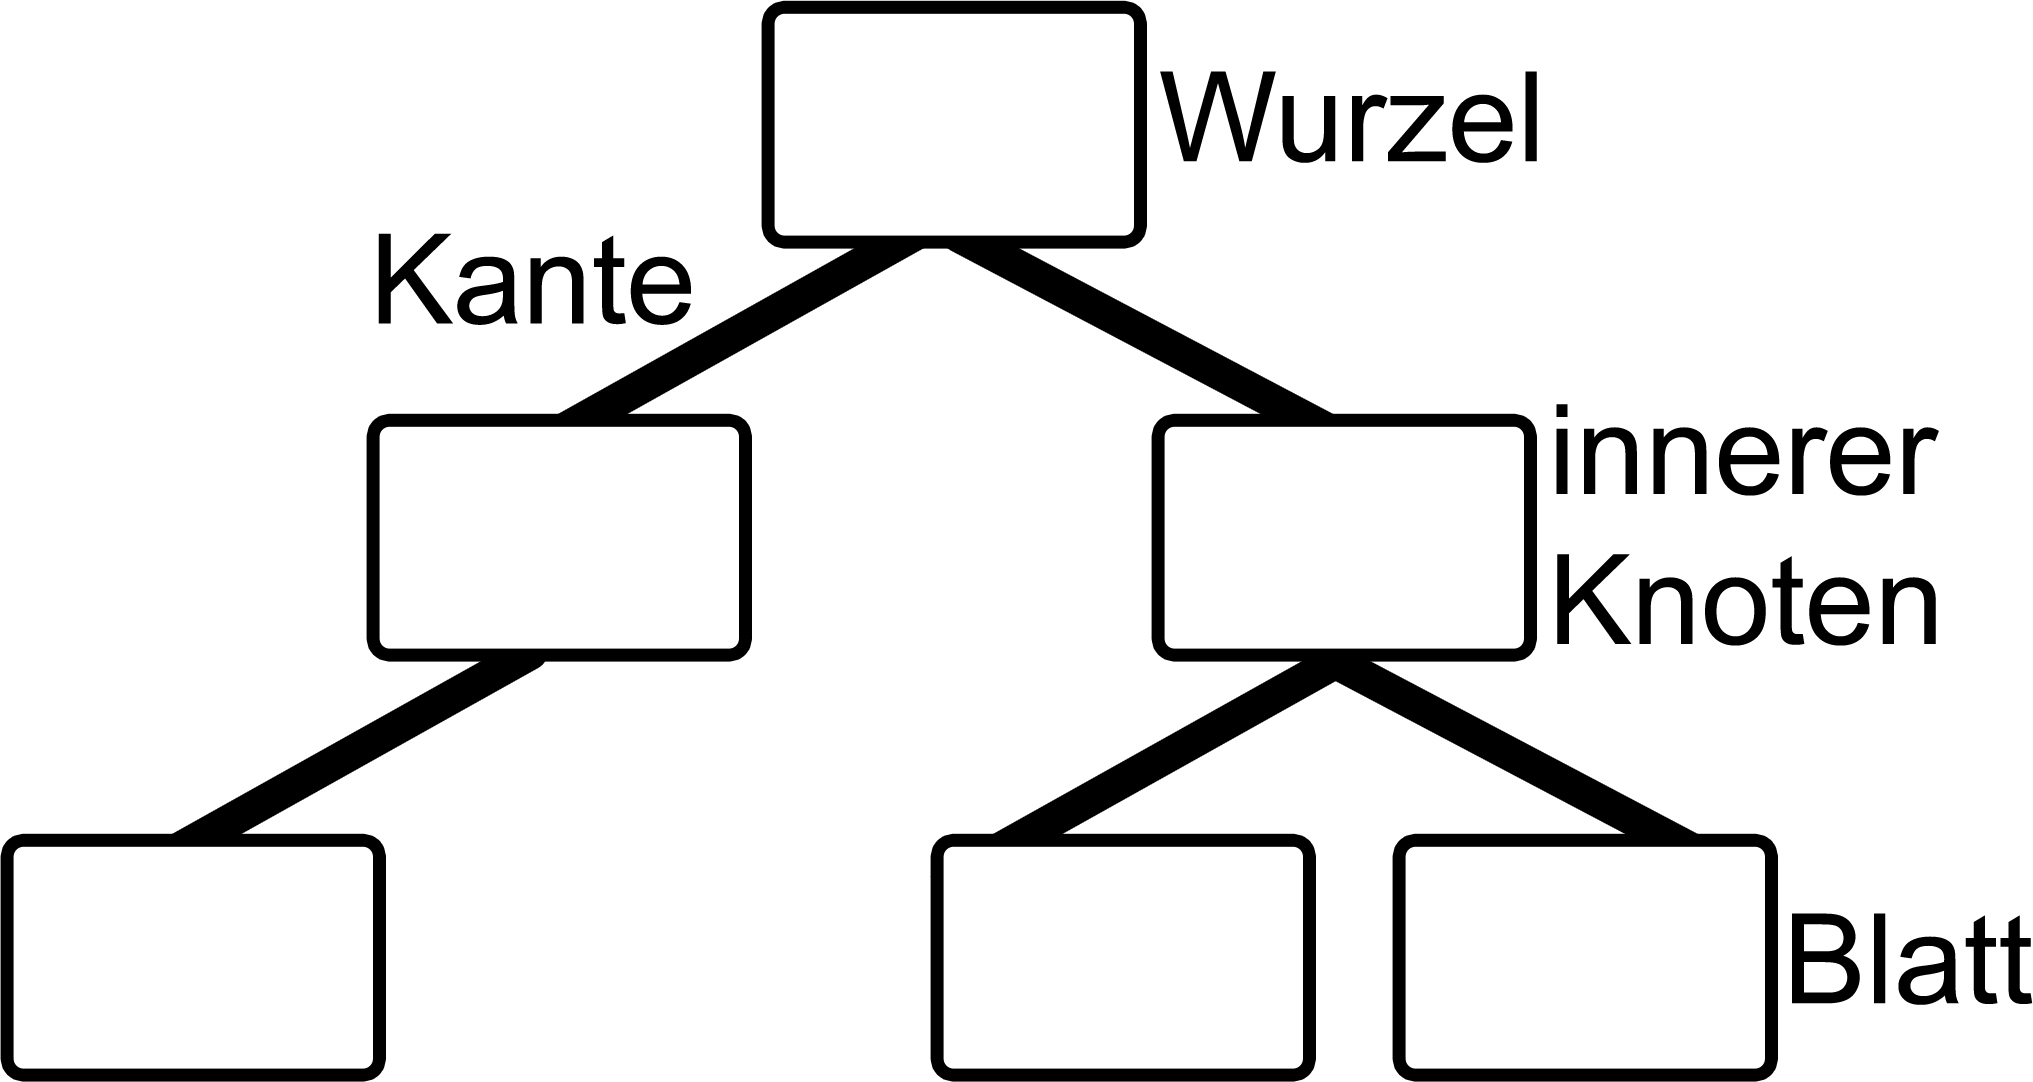
\includegraphics[width=\linewidth]{images/binarytree.jpg}
  \caption{Baumstruktur}
  \captionsource{Von Mhombach - Eigenes Werk, CC BY-SA 3.0, https://commons.wikimedia.org/w/index.php?curid=29981537}
  \label{fig:binarytree}
\end{figure}

Eine Baumstruktur (\ref{fig:binarytree}) besteht aus einem Wurzel-knoten,
welcher mithilfe von Kanten ``Kind knoten'' oder auch ``innere Knoten'' besitzen
kann. Hat ein Knoten keine ``Kinder'', wird er als ``Blatt'' bezeichnet.
Baumstrukturen sind für die Darstellung von Daten aufgrund ihrer einfachen
Gestaltung vorteilhaft. Eine Baumstruktur kann sehr leicht mithilfe von
rekursiven Funktionen durchlaufen werden, da ein Knoten immer genau ein
``Elternteil'' und eine Liste von ``Kindern'' hat.

\section{\acl{VDOM}}
\subsection{Definition}

Ein \ac{VDOM} ist eine Repräsentation eines \ac{DOM} welche durch arbiträre
Datenstrukturen abgebildet werden kann. Eine häufige Implementation ist durch
Javascript-Objekte, welche die Daten des \ac{DOM} abbilden.

\subsection{Motivation}

Oft wird ein \ac{VDOM} verwendet, da aus manipulation der Daten automatisch eine
Änderung im \ac{DOM} abgebildet werden kann, und somit der Entwickler lediglich
die Änderung der Daten bedenken muss.

\subsection{Nachteile}

Eine Repräsentation des \ac{DOM} als \ac{VDOM} führt zwangsläufig dazu, dass die
Struktur des \ac{DOM} doppelt vorhanden ist. Desweiteren ist das finden der
Änderungen zwischen \ac{DOM} und \ac{VDOM} nicht trivial und langsamer als eine
``direkte'' Änderung der Daten im \ac{DOM}. Weiterhin muss der Web-Browser
zusätzlich zum finden der Änderungen zwischen \ac{DOM} und \ac{VDOM} immer
die \ac{DOM}-\ac{API} Aufrufe ausführen.

\section{\acl{SPA}}
Eine \ac{SPA} beschreibt eine Web-Applikation, die auf einer Webseite abgebildet ist. Dies wird realisiert, indem die gesamte Präsentationslogik, im Kontrast zu traditionellen Webanwendungen, im Browser implementiert wird.\cite{SPA} 
\subsection{Unterscheidung}
\subsubsection{Traditionelle Webanwendung}
\begin{figure}
  \begin{center}
    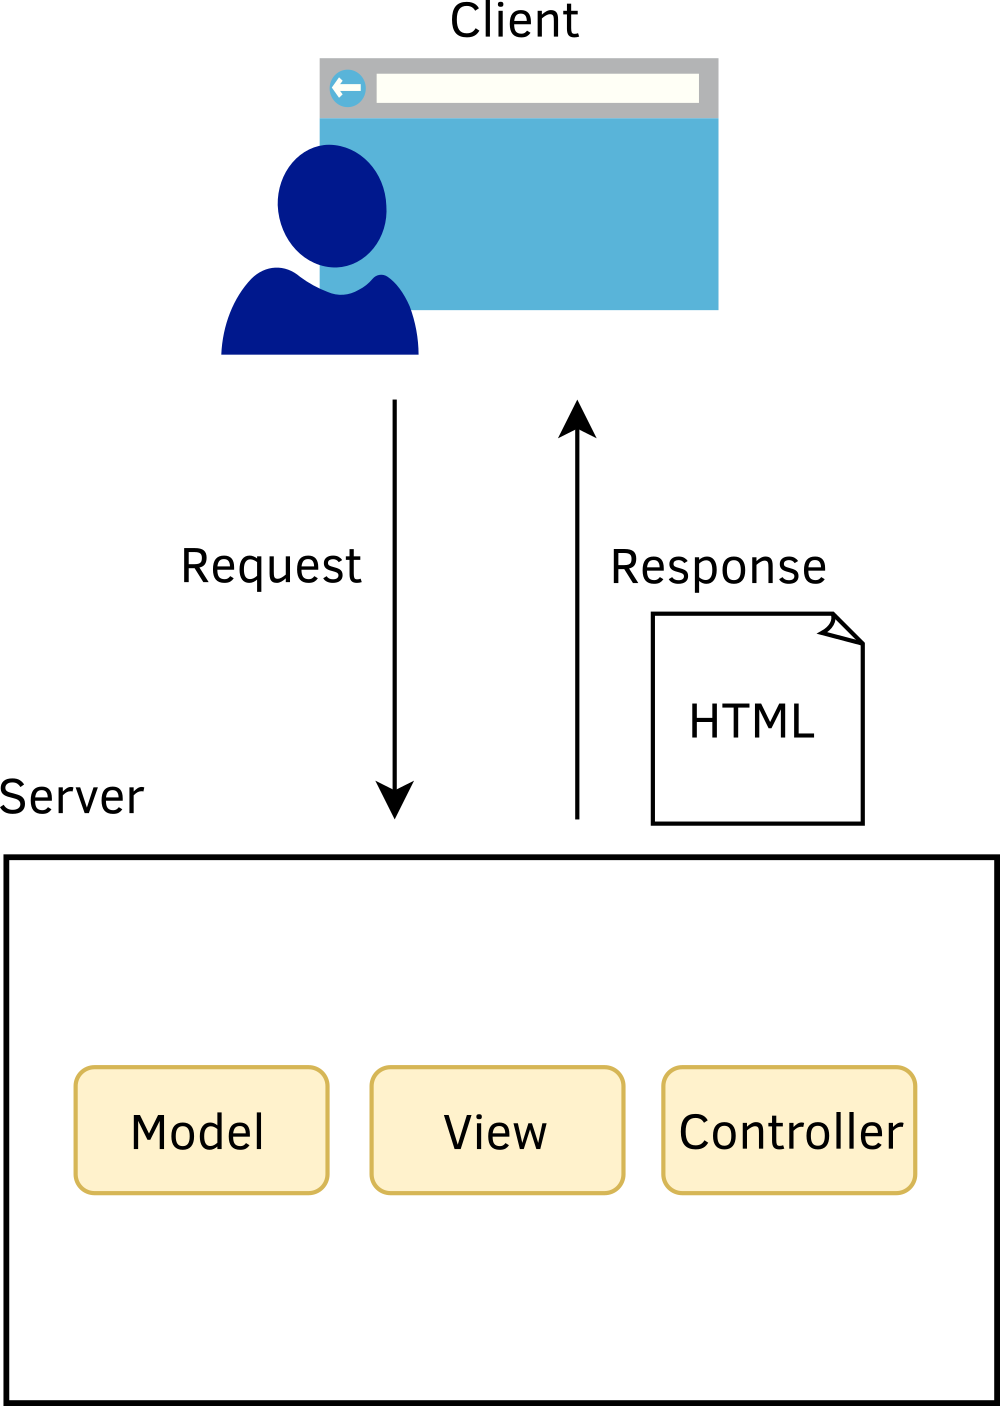
\includegraphics[scale=1]{images/traditonal_web_app.png}
  \end{center}
  \caption{Traditionelle Web Anwendung}
  \captionsource{Eigenes Werk}
  \label{fig:tradweb}
\end{figure}
Traditionelle Webanwendungen (siehe Abbildung \ref{fig:tradweb}) lösen bei jeder Anfrage des Nutzers einen Roundtrip \footnote{Senden einer Anfrage an einen Server und Erhalt der entsprechenden Antwort} aus zum Server aus.\\
Server-seitig wird der Request von einem Controller entgegengenommen. Dieser agiert mit dem Model, welches die benötigten Daten liefert (beispielsweise durch eine Anfrage an eine Datenbank). Die Logik im Controller bestimmt anschließend das benötigte View und füllt dieses mit Daten.\\
Der Server antwortet mit einem \ac{HTML} Dokument und der Browser stellt dies nach einer Aktualisierung der gesamten Webseite dar.
\subsubsection{\acl{SPA}}
\begin{figure}
  \begin{center}
    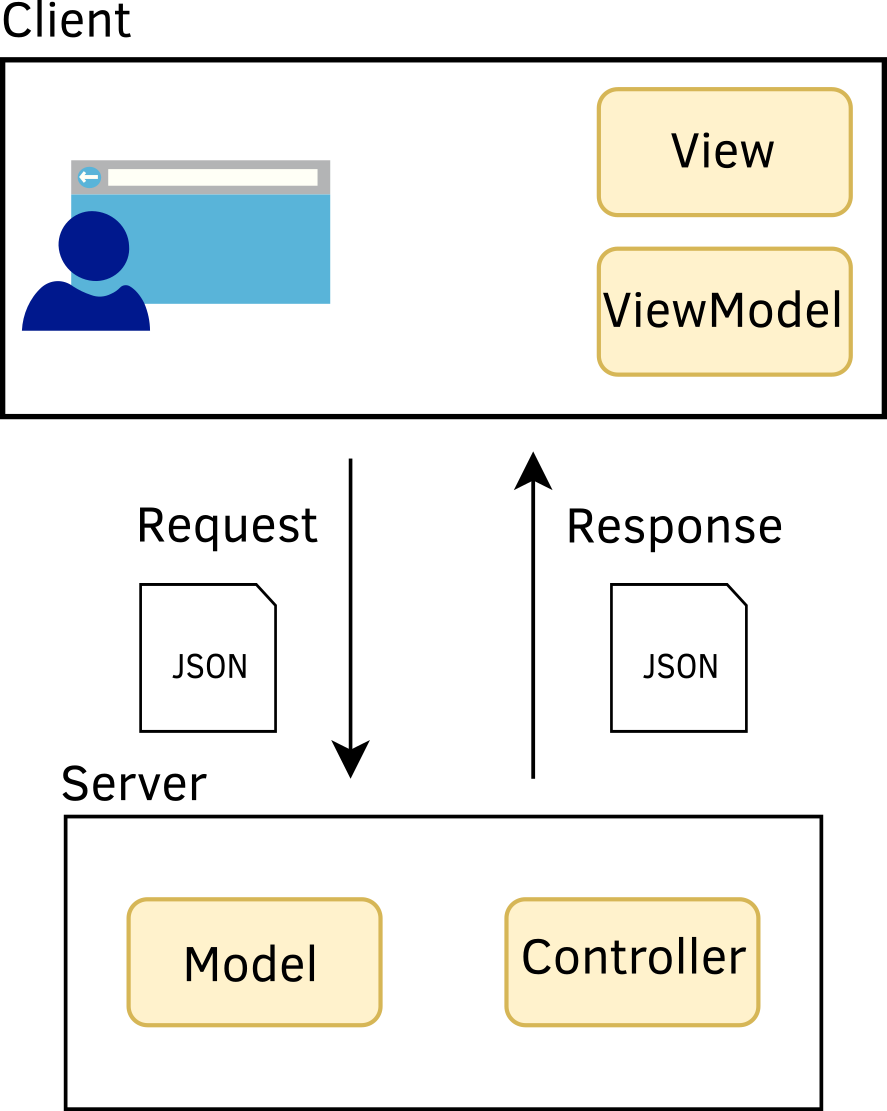
\includegraphics[scale=1.5]{images/spa_web_app.png}
  \end{center}
  \caption{\acl{SPA}}
  \captionsource{Eigenes Werk}
  \label{fig:spaweb}
\end{figure}
Bei einer \ac{SPA} hingegen wird die gesamte View Logik in den Client verlagert
(siehe Abbildung \ref{fig:spaweb}). Die Kommunikation mit dem Server reduziert
sich bei dieser Architektur auf reinen Austausch von Daten.\\
Eine Aktion des Nutzers, beispielsweise ein Klick auf einen Button, wird behandelt indem das
View die Aktion an das Viewmodel weiterleitet. Das Viewmodel aktualisiert den
lokalen Zustand (State) der Anwendungen und stell bei Bedarf eine Anfrage an den Server um Daten auszutauschen und aktualisiert anschließend
das View.\\
Dies hat diverse Auswirkungen auf die Anwendung: 
\begin{description}
  \item[Keine Aktualisierungen der gesamten Seite]In einer \ac{SPA} werden Views
    nicht als gesamte \ac{HTML} Seite abgebildet. Vielmehr ist ein View als ein
    Teil des \ac{DOM} anzusehen, welches zum richtigen Zeitpunkt mit dem
    vorhergegangen View ausgetauscht wird. Nach dem initialen Laden der Seite
    gibt es keine weiteren Aktualisierungen dieser.\\
    Aus Sicht der \ac{UX}
    gleicht dies mehr einer nativen Smartphone App als einer Webseite. Dies
    führt zu einer vertrauteren Umgebung, insbesondere wenn die Anwendung auf
    einem Smartphone oder Tablet benutzt wird.
  \item[Trennung von Client und Server]Durch die Verlagerung der
    View Logik wird eine klare Abgrenzung zwischen Client und Server erreicht.
    Die Kommunikation wird durch eine \ac{REST} Spezifikation ausgedrückt und
    somit ist sowohl der Client als auch der Server leicht austuschbar. Diese
    Entkopplung ist bekannt unter dem Ausdruck ``single responsibility principle''\cite{cleancode}.
\end{description}

\section{Datenstrukturen}
\subsection{\acl{DBMS}}
\subsection{\acl{ERM}}
\section{Plug-ins}
Modularität war von Anfang an ein wichtiger Gesichtspunkt bei der Entwicklung
von Chromstahl. Es sollte möglich sein, das \ac{CMS} effizient an neue Aufgaben
anzupassen, beispielsweise für ein Video Portal. Eine solche Modularität lässt
sich über Plug-ins realisieren.
\subsection{Definition}
Ein Plug-in (auch Add-on genannt) ist eine Komponente die eine spezielle
Funktion zu einer bestehenden Software
hinzufügt.\footnote{https://en.wikipedia.org/wiki/Plug-in\_(computing)}. Die
Software stellt \ac{API}s bereit, gegen welche ein Plug-in entwickelt werden kann.
\subsection{Implementationsansätze}
% TODO: flesh this out
Zu Beginn des Projektes wurden zwei Ansätze zur Implementierung von Plug-ins für
Chromstahl konzipiert. Diese werden im folgenden erläutert und im späteren
Verlauft dieser Arbeit konkret behandelt.
\begin{description}
\item[Dynamisch]{Zum einen gibt es den Ansatz, Plug-ins dynamisch zu laden. Dies
  bedeutet, dass bei Start der Anwendung Plug-ins gesucht und entsprechend
  gealden werden. Dies führt zu einer höheren Flexibilität beim Benutzen der
  Anwendung, bringt allerdings auch einen höheren Entwicklungsaufwand mitsich}
\item[Statisch]{Der zweite Ansatz ist das statische Laden von Plug-ins. Hierbei
    werden Plug-ins zur Kompilierzeit aufgelöst. Dies führt zu einem Kompilat,
    welches alle Plug-ins gebündelt enthält und somit verlässlicher
    bereitzustellen ist. Allerdings zieht eine Änderung an den Plug-ins der
    Anwendung ein erneutes Kompilieren mitsich}
\end{description}
% LocalWords:  Superset
